%&pdflatex
\documentclass[mathserif]{beamer} %, handout
\usetheme[progressbar=foot]{metropolis}
\setbeamertemplate{caption*}[numbered]

\usepackage[utf8x]{inputenc}
\usepackage[T2A]{fontenc}
\usepackage[english,russian]{babel}

\usepackage{amssymb, amsmath, amsfonts, mathtools, mathrsfs}
\usepackage[normalem]{ulem} % for sout
\usepackage{comment}

\AtBeginSubsection{
\frame[plain,c]{\subsectionpage}
}

\defbeamertemplate{subsection page}{simple}{
  \centering
  \usebeamercolor[fg]{subsection title}
  \usebeamerfont{subsection title}
  \insertsubsection\\
}
\setbeamertemplate{subsection page}[simple]

\title{Кинетическое уравнение Больцмана: функциональный, асимптотический и численный анализ}
\author{Рогозин Олег Анатольевич}
\institute{
    Вычислительный центр ФИЦ ИУ РАН
}
\date{\today}

\newcommand{\Kn}{\mathrm{Kn}}
\newcommand{\St}{\mathrm{St}}
\newcommand{\Ma}{\mathrm{Ma}}
\newcommand{\loc}{\mathrm{loc}}
\newcommand{\eqdef}{\overset{\mathrm{def}}{=}}
\newcommand{\dd}{\:\mathrm{d}}
\newcommand{\pder}[2][]{\partial_{#2}{#1}}
\newcommand{\pderdual}[2][]{\partial_{#2^2}{#1}}
\newcommand{\pderder}[2][]{\frac{\partial^2 #1}{\partial #2^2}}
\newcommand{\Pder}[2][]{\partial#1/\partial#2}
\newcommand{\dxi}{\dd\xi}
\newcommand{\OO}[1]{O(#1)}
\newcommand{\Set}[2]{\{\,{#1}:{#2}\,\}}
\newcommand{\xoverbrace}[2][\vphantom{\int}]{\overbrace{#1#2}}
\newcommand{\Cite}[2][]{\alert{\textsc{#2 #1}}}

\begin{document}

\frame{\titlepage}

\begin{frame}
  \frametitle{Содержание}
  \linespread{0.8}
  \tableofcontents
\end{frame}

\section{Функциональный анализ}

\begin{frame}
    \frametitle{Функция распределения}
    Microscopic description % минимальные предположения
    \begin{equation*}
        f(t,x,\xi): \mathbb{R}_+\times\Omega\times\mathbb{R}^N\mapsto\mathbb{R}_+
        \quad (\Omega\subset\mathbb{R}^N),
    \end{equation*}
    \begin{equation*}
        f(t,\cdot,\cdot) \in L^1_\loc(\Omega; L^1(\mathbb{R}^N)).
    \end{equation*}
    Macroscopic quantities % часто более гладкие, чем ФР
    \begin{equation*}
        \begin{gathered}
        \rho = \int_{\mathbb{R}^N} f\dxi, \quad v = \frac1\rho\int_{\mathbb{R}^N} \xi f\dxi, \\
        T = \frac1{N\rho}\int_{\mathbb{R}^N} \left(|\xi|^2 - |v|^2\right) f\dxi.
        \end{gathered}
    \end{equation*}
\end{frame}

\subsection{Уравнение Больцмана и его особенности}

\begin{frame}
    \frametitle{Уравнение Больцмана}
    \begin{equation*}
        \pder[f]{t} + \xi\cdot\pder[f]{x} = Q(f,f).
    \end{equation*}

    \begin{itemize}
        \item \(\xi\cdot\pder{x}\) "--- transport operator (conservative)
        \item \(Q(f,f)\) "--- collisional operator (dissipative)
    \end{itemize}

    \pause
    Derivation from the Liouville equation in the Boltzmann--Grad limit: % (low-density)
    \[ nr^{N-1}=\OO{1}, \quad n\to\infty\]\vspace{-20pt}
    \begin{itemize}
        \item \Cite[1958]{Grad}: correct limiting procedure for HS
        \item \Cite[1972]{Cercignani}: rigorous formulation (need \(\exists!\) theorems)
        \item \Cite[1975]{Lanford}: rigorous result for short times and HS
        \item \Cite[1986]{Illner, Pulvirenti}: full result for rare cloud of gas expanding in the vacuum
        \item \Cite[2013]{Gallangher, Saint-Raymond, Texier}: recollisions, smooth positive short-range potentials
    \end{itemize}
\end{frame}

\begin{frame}
    \frametitle{Столкновительный интеграл}
    \begin{gather*}
        Q(f,f)(t,x,\xi) \eqdef \int_{\mathbb{R}^N}\dxi_* \int_{S^{N-1}} \dd\sigma
        \overbrace{B(\xi-\xi_*,\sigma)}^\text{collisional kernel}
        \Big( \overbrace{f'f'_*}^\text{gain} - \overbrace{ff_*}^\text{loss} \Big), \\
        \xi' = \dfrac{\xi+\xi_*}2 + \dfrac{|\xi-\xi_*|}2\sigma, \quad
        \xi'_* = \dfrac{\xi+\xi_*}2 + \dfrac{|\xi-\xi_*|}2\sigma.
    \end{gather*}

    \pause
    \begin{gather*}
        V(r)\sim r^{1-s} \:\implies\: \sin^{N-1}\theta B(|z|,\cos\theta) \sim |z|^\gamma \theta^{-1-\nu} \quad(z=\xi-\xi_*), \\
        \quad \gamma = \dfrac{s-5}{s-1}\in[-3,1], \quad \nu = \dfrac2{s-1}\in[0,2].
    \end{gather*}
    \vspace{-20pt}
    \begin{itemize}
        \item hard spheres: \(s=+\infty,\quad\gamma=1,\quad\nu=0 \quad\implies\quad B=|z|\)
        \item hard potentials: \(\gamma>0\)
        \item Maxwell: \(s=5,\quad\gamma=0,\quad\nu=1/2\)
        \item soft potentials: \(\gamma<0\)
        \item Coulomb: \(s=2,\quad\gamma=-3,\quad\nu=2\) \(\quad\longrightarrow\quad\) Landau equation
    \end{itemize}

\end{frame}

\begin{frame}
    \frametitle{Симметрии и H-теорема Больцмана}
    Weak formulation:
    \begin{equation*}
        \int_{\mathbb{R}^N} Q(f,f)\varphi = \frac14 \int_{\mathbb{R}^N} Q(f,f) (\varphi + \varphi_* - \varphi' - \varphi'_*).
    \end{equation*}
    \pause
    Lyapunov functional or H-functional or negative entropy:
    \begin{equation*}
        H(f) \eqdef \int_{\Omega\times\mathbb{R}^N} f\log{f} \xrightarrow{t\to\infty} \min.
    \end{equation*}
    Entropy production functional:
    \begin{equation*}
        D(f) \eqdef -\int_{\mathbb{R}^N} Q\log{f} = \frac14\int_{\mathbb{R}^{2N}\times S^{N-1}}
        B\left( f'f'_* - ff_* \right) \log\frac{f'f'_*}{ff_*} \geq 0.
    \end{equation*}
    H-theorem:
    \begin{equation*}
        \pder[H]{t} = - \int_\Omega D.
    \end{equation*}
\end{frame}

\subsection{Существование и свойства решений}

\begin{frame}
    \frametitle{Теория жёстких усечённых потенциалов}
    \Cite[1958]{Grad}: Grad's angular cutoff = short-range assumption
    \[ B\in L^1_\loc. \]
    Existence and uniqueness of \(\pder[f]{t} = Q(f,f)\) in \(L^1\):
    \begin{itemize}
        \item \Cite[1933]{Carleman}, \Cite[1962]{Povzner}: hard spheres
        \item \Cite[1955]{Morgenstern}: Maxwellian molecules
        \item \Cite[1972]{Arkeryd}: hard potentials
        \item \Cite[1999]{Mischler, Wennberg}: optimal result (\(f_0\in L^1_2\), \sout{\(L\log{L}\)})\!\!\!\!\!\!\!\!\!\!
        \[ L^1_q \eqdef \Set{f}{\int_{\mathbb{R}^N} f(1+|\xi|^q) < +\infty}. \]
        \item \Cite[1999]{Wennberg}: nonuniqueness result (increasing energy)
    \end{itemize}
\end{frame}

\begin{frame}
    \frametitle{Теория жёстких усечённых потенциалов}
    \begin{itemize}
        \item \Cite[1999]{Mischler, Wennberg}: moment bounds
        \[ \forall q\geq2: \sup_{t\geq t_0>0} \int_{\mathbb{R}^N} f_t (1+|\xi|^q) \]
        \item \Cite[1997]{Pulvirenti, Wennberg}: Maxwellian lower bound
        \[ \forall t_0>0, \exists K_0,A_0>0: f_{t>0}(\xi) \geq K_0\exp\left( -A_0 |\xi|^2\right) \]
        \item \Cite[2009]{Gamba, Panferov, Villani}: Maxwellian upper bound \!\!\!\!\!
        \[ f_0 \leq M_0(\xi) \implies f_t \leq M(\xi)\]
        \item \Cite[2004]{Mouhot, Villani}: regularization theory (gain term)
        \begin{gather*}
            \forall s\geq0,q\geq0,t_0>0,k>0 : f_{t\geq t_0} = f^S_t + f^R_t, \\
            \sup_{t\geq t_0} \|f^S_t\|_{H^s_q\cap L_2^1} < +\infty,
            \quad \|f^R_t\|_{L_k^1} = \OO{e^{-\lambda t}}
        \end{gather*}
    \end{itemize}
\end{frame}

\begin{frame}
    \frametitle{Теория мягких потенциалов}
    \begin{itemize}
        \item \Cite[1981]{Arkeryd}, \Cite[1997]{Goudon}: weak solutions (\(\gamma\geq-2\))
        \[ (\varphi + \varphi_* - \varphi' - \varphi'_*) \sim |z|^2 \]
        \item \Cite[1999]{Villani}: H-solutions (\(-4<\gamma<-2\))
        \begin{gather*}
            D(f) \geq \int_{\mathbb{R}^{2N}\times S^{N-1}} B(|z|, \sigma) \left(\sqrt{f'f'_*} - \sqrt{ff_*}\right)^2, \\
            \left| \int_{\mathbb{R}^N} Q(f,f)\varphi \right| \leq \frac12
            \sqrt{ D(f) \int Bff_* (\varphi + \varphi_* - \varphi' - \varphi'_*)^2 }
        \end{gather*}
        \item Bad estimates on moments:
        \[ \forall q>2: \quad\int_{\mathbb{R}^N} f_t |\xi|^q < C(1+t) \]
    \end{itemize}
\end{frame}

\begin{frame}
    \frametitle{Теория неусечённых потенциалов}
    Nonintegrable angular singularity due to grazing collisions (\(\theta\to0\)):
    \[ \int_0^{\frac\pi2} b(\cos\theta)\sin^{N-2}\theta\dd\theta = +\infty \]
    \vspace{-20pt}
    \begin{itemize}
        \item \Cite[2000]{Alexandre, Desvillettes, Villani, Wennberg}:
        \begin{gather*}
            \text{collisional} \:\longrightarrow\: \text{diffusive--collisional} \\
            D(g,f) \eqdef -\int_{\mathbb{R}^N} Q(g,f)\log{f} \geq C_1\|\sqrt{f}\|^2_{H^\frac\nu2} - C_2\|f\|_{L^1_2}\|g\|_{L^1_2}, \\
            \implies Q \sim -(-\Delta)^\frac\nu2
        \end{gather*}
        \item \Cite[2004]{Desvillettes, Wennberg}: Schwartz space \(\mathscr{S}\)
        \[ f \in L^\infty\left([t_0>0,+\infty); \mathscr{S}(\mathbb{R}^N)\right) \]
        \item \Cite[2009]{Desvillettes, Mouhot}: uniqueness
        \[ \forall\nu\in(0,2): \quad\exists! f_t\in W_q^{1,1} \]
    \end{itemize}
\end{frame}


\begin{frame}
    \frametitle{Пространственно-неоднородная задача}
    \begin{itemize}
        \item \Cite[1985]{Golse, Perthame, Sentis}: velocity-averaging lemmas\!\!\!\!\!\!
        \[ f\in L^2_{t,x,\xi}, Q\in L^2_{t,x}(H_\xi^s) \implies
        \forall\varphi\in C^\infty: \int_{\mathbb{R}^N} f\varphi\in H_{t,x}^{\frac1{2(1+s)}} \]
        % macroscopic observables enjoy some smoothness properties even when the distribution function itself does not
        \item \Cite[1989]{DiPerna, Lions}: \(\exists\) renormalized solutions in \(L^1\)
        \[ \pder[\beta(f)]{t} + \xi\cdot\pder[\beta(f)]{x} = \beta'(f)Q(f,f) \]
        \item \Cite[2002]{Alexandre, Villani}: extension for non-cutoff case
    \end{itemize}
    \begin{itemize}
        \item for \(\beta'(f) \leq C/(1+f)\) we expect \(\beta'(f)Q(f,f)\) is sublinear
        \item only existence! (stability result)
        \item \sout{uniqueness, energy conservation, moment estimates, positivity, trend to equilibrium}
        \item like weak solutions for Navier--Stokes due to \Cite[1934]{Leray}
    \end{itemize}
\end{frame}

\subsection{Сходимость к равновесию}

\begin{frame}
    \frametitle{Седрик Виллани}
    \begin{columns}
    \begin{column}{0.2\textwidth}
       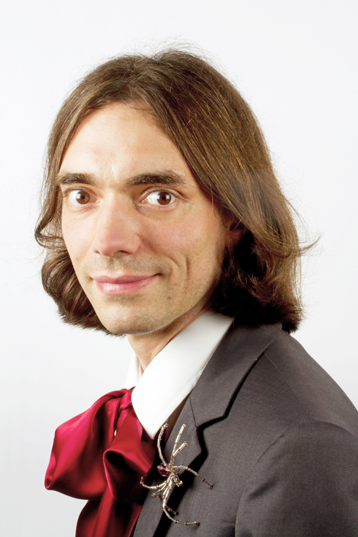
\includegraphics{photos/villani3}
    \end{column}
    \begin{column}{0.8\textwidth}
        \begin{itemize}
            \item \Cite{1998}: PhD Thesis (advisor P.-L. Lions)
            \item \Cite{2000}: Habilitation dissertation
            \item with \Cite[2000]{Alexandre, Desvillettes, Wennberg}: non-cutoff theory
            \item with \Cite[1999]{Toscani}; \Cite{2000, 2003}: Cercignani's conjecture
            \item with \Cite[2002]{Alexandre}: DiPerna--Lions for non-cutoff
            \item with \Cite[2005]{Desvillettes}: trend to equilibrium
            \item \Cite{2009}: Hypercoercivity
            \item \Cite{2010}: Fields medal
        \end{itemize}
    \end{column}
    \end{columns}


\end{frame}

\begin{frame}
    \frametitle{Гипотеза Черчиньяни}
    \begin{itemize}
        \item \Cite[1982]{Cercignani} conjectured exponential decay
        \[ D(f) \geq \lambda(f_0) H(f|M^f), \quad  H(f|M^f) \eqdef H(f) - H(M^f) \]
        \item \Cite[1984]{Bobylev}, \Cite[1997]{Wennberg}: some counterexamples
        \item \Cite[1999]{Bobylev, Cercignani}: false for physical solutions
        \item \Cite[1992, 1994]{Carlen, Carvalho}: \( D(f) \geq \Phi(H(f|M^f)) \)
        \item \Cite[1999]{Toscani, Villani}: optimal result for hard \((1+|z|^\gamma)\)
        \[ \forall\varepsilon>0: D(f) \geq C_\varepsilon(f) H(f|M^f)^{1+\varepsilon}\]
        \item \Cite[2000, 2003]{Villani}: extended result \(\OO{t^{-\infty}}\)
    \end{itemize}
\end{frame}

\begin{frame}
    \frametitle{Сходимость к равновесию}
    \Cite[2005]{Desvillettes, Villani}, \Cite[2009]{Villani}
    \begin{gather*}
        \left.\frac{\dd^2}{\dd{t}^2}\right|_{t=0} \| f-M^f_{\rho v T} \| \geq K\left(
            \int |\nabla{T}|^2 + \int |\{\nabla{v}\}|^2 \right), \\
        \left.\frac{\dd^2}{\dd{t}^2}\right|_{t=0} \| f-M^f_{\rho 0 1} \| \geq K\left(
            \int |\nabla{\rho}|^2 \right)
    \end{gather*}
    \hspace*{-20pt}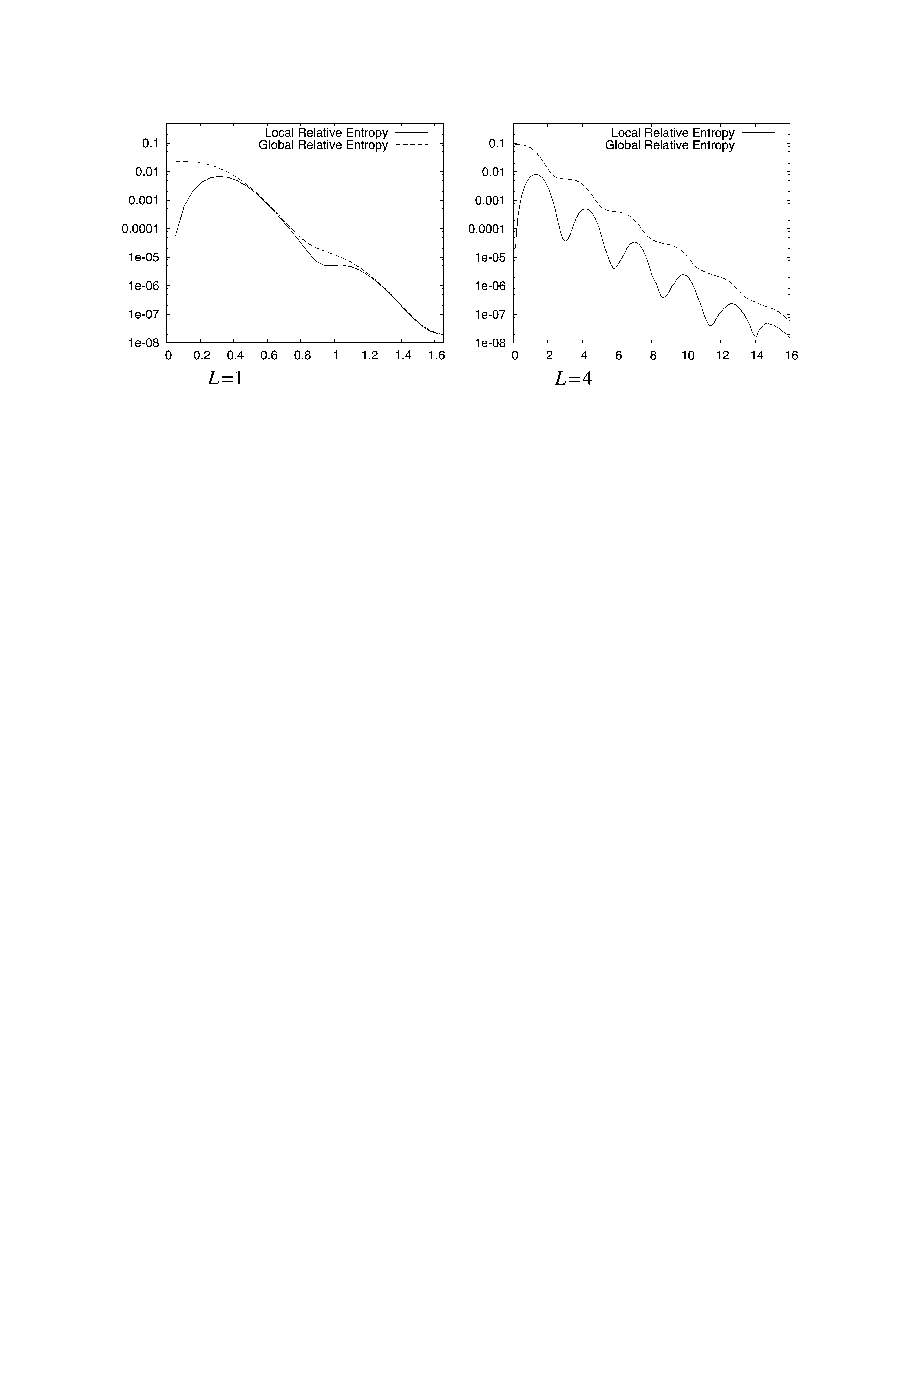
\includegraphics{cutted/filbet}
\end{frame}

\begin{comment}
\begin{frame}
    \frametitle{Классические решения}
    % Ukai, Guo
    % spectral gap (no Caflisch)
    % Mouhot, Strain -> Gressman, Strain
    \begin{equation*}
        \pder[f]{t} + \mathcal{B}f = \mathcal{C}f.
    \end{equation*}
\end{frame}
\end{comment}

\section{Асимптотический анализ}

\subsection{Гидродинамические пределы}

\begin{frame}
    \frametitle{Строгие результаты}
    \begin{itemize}
        \item \Cite[1912]{Hilbert}, \Cite[1917]{Enskog}: formal expansions
        \item \Cite[2004, 2008]{Golse, Saint-Raymond}: incompressible Navier--Stokes limit for DiPerna--Lions
        \item incompressible Euler limit: lack of regularity estimates
        \item compressible Euler limit:\newline
        how entropy production concentrates on shocks/discontinuites
    \end{itemize}
\end{frame}

\begin{frame}
    \frametitle{Числа Кнудсена и Струхаля}
    \[ \St \pder[f]{t} + \xi\cdot\pder[f]{x} = \frac1{\Kn} Q(f,f)\]
    \begin{itemize}
        \item fluid-dynamic limit: \(\Kn\to0\), classification due to \(\St\)
        \item initial layer \(\St = \OO{\Kn^{-1}}\)
        \item Euler (inviscid) region \(\St = \OO{1}\)
        \item diffusion (viscous) region \(\St = \OO{\Kn}\)
    \end{itemize}
\end{frame}

%%% Saint-Raymond
\subsection{Классификация кинетических слоёв}

\begin{frame}
    \frametitle{Асимптотический анализ для \(\Ma = \OO{1}\)}
   	\begin{columns}
		\column{.55\textwidth}
		\begin{center}
		    \vspace{-27pt}
			\includegraphics[width=\textwidth]{tikz/layers}
		\end{center}
		\column{.5\textwidth}
		\vspace{-10pt}
		\begin{itemize}
			\item область невязкого течения \[ \pder[f]{x_i}n_i = \OO{f} \]
			\item вязкий пограничный слой \[ \sqrt{k}\pder[f]{x_i}n_i = \OO{f} \]
			\item cлой Кнудсена \[ k\pder[f]{x_i}n_i = \OO{f} \]
			\item слой Соне [Sone 1973] \[ \pder[f]{x_i}n_i \to \infty \]
		\end{itemize}
	\end{columns}
\end{frame}

%%% Sone's asymptotic theory
%%% Maslova-Bardos theorem

\section{Численный анализ}

\subsection{Поиск консервативных методов}

\begin{frame}
    \frametitle{Численные методы}
    Diversity:
    \begin{itemize}
        \item stochastic models (DSMC)
        \item discrete-velocity models
        \item discrete-velocity methods
        \item spectral methods (Fourier, wavelet,...)
    \end{itemize}
    Key properties:
    \begin{itemize}
        \item conservation of mass, momentum, kinetic energy
        \item H-theorem
        \item positivity
    \end{itemize}
\end{frame}

\begin{frame}
    \frametitle{Дискретизация пространства скоростей}
    \begin{center}
    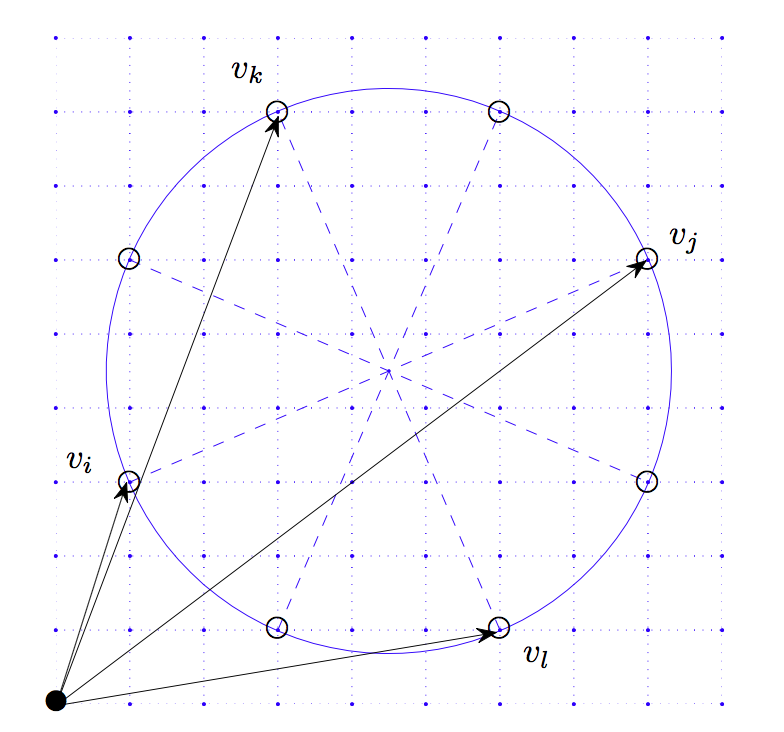
\includegraphics[width=0.7\textwidth]{cutted/dimarco}
    \end{center}
\end{frame}

\begin{frame}
    \frametitle{Дискретизация пространства скоростей}
    \begin{itemize}
        \item \Cite[1997]{Palczewski, Schneider, Bobylev}: consistency of DV models
        \item \Cite[1997]{Mischler}: convergence to DiPerna--Lions
    \end{itemize}
    Very bad rate of convergence \(\:\implies\:\) need regularization technique
    \begin{itemize}
        \item \Cite[1998]{Buet, Cordier, Degond}: mollification of collision sphere or masses
        \item \Cite[1998]{Tcheremissine}: projective method
    \end{itemize}
\end{frame}

\end{document}
